\documentclass[12pt,a4paper]{report}
\usepackage{fontspec}  % 字体配置包（xelatex必需）
\usepackage[UTF8]{ctex}  % 中文支持，使用默认字体集
\usepackage{geometry}
\usepackage{amsmath}
\usepackage{graphicx}
\usepackage{booktabs}
\usepackage{array}
\usepackage{setspace}
\usepackage{indentfirst}
\usepackage{fancyhdr}
\usepackage{lastpage}
\usepackage{cite}
\usepackage{enumitem}
\usepackage{chemfig}  % 化学结构式
\usepackage{tabularx}  % 表格扩展
\usepackage{titlesec}  % 标题格式控制
\usepackage{caption}   % 图表标题格式控制
\usepackage[normalem]{ulem}  % 下划线支持
\usepackage[unicode=true,colorlinks=true,linkcolor=blue,citecolor=blue,urlcolor=blue,bookmarks=true,bookmarksnumbered=true]{hyperref}

% 页面设置 - 按照湖南大学规范
\geometry{top=30mm,bottom=25mm,left=30mm,right=20mm,headheight=15pt}
\setstretch{1.5}  % 1.5倍行距（按照规范3.5.2）
\setlength{\parindent}{2em}  % 首行缩进

% 页眉页脚 - 按照湖南大学规范
\pagestyle{fancy}
\fancyhf{}
\renewcommand{\headrule}{
    \hrule height 1.2pt width\headwidth
    \vskip 0.6pt
    \hrule height 0.7pt width\headwidth
}
\fancyhead[C]{\zihao{-5} 湖南大学本科生毕业论文}
\fancyfoot[C]{\zihao{-5} \thepage}

% 封面不显示页码
\fancypagestyle{noheader}{
    \fancyhf{}
    \renewcommand{\headrulewidth}{0pt}
}

% 修改 chapter 的 plain 样式，使其也显示页眉
\fancypagestyle{plain}{
    \fancyhf{}
    \renewcommand{\headrule}{
        \hrule height 1.2pt width\headwidth
        \vskip 0.6pt
        \hrule height 0.7pt width\headwidth
    }
    \fancyhead[C]{\zihao{-5} 湖南大学本科生毕业论文}
    \fancyfoot[C]{\zihao{-5} \thepage}
}

% 定义字体字号命令
\newcommand{\sizeFive}{\fontsize{10.5pt}{15pt}\selectfont}  % 五号
\newcommand{\sizeFour}{\fontsize{14pt}{20pt}\selectfont}    % 四号
\newcommand{\sizeFourl}{\fontsize{12pt}{15pt}\selectfont}   % 小四
\newcommand{\sizeThree}{\fontsize{16pt}{20pt}\selectfont}   % 三号
\newcommand{\sizeThreel}{\fontsize{15pt}{20pt}\selectfont}  % 小三
\newcommand{\sizeTwo}{\fontsize{22pt}{28pt}\selectfont}     % 二号
\newcommand{\sizeTwol}{\fontsize{18pt}{22pt}\selectfont}    % 小二
\newcommand{\sizeOne}{\fontsize{26pt}{36pt}\selectfont}    % 一号

% 章节标题格式 - 按照湖南大学规范
% 章标题:三号黑体
\titleformat{\chapter}{\heiti\sizeThree}{\thechapter}{1em}{}
\titlespacing{\chapter}{0pt}{0pt}{2pt}

% 节标题:小四号黑体,段前段后各0.5行(7.5pt)
\titleformat{\section}{\heiti\sizeFourl}{\thesection}{1em}{}
\titlespacing{\section}{0pt}{7.5pt}{7.5pt}

% 条标题:小四号黑体,段前段后各0.5行(7.5pt)
\titleformat{\subsection}{\heiti\sizeFourl}{\thesubsection}{1em}{}
\titlespacing{\subsection}{0pt}{7.5pt}{7.5pt}

% 款标题:小四号黑体,段前段后各0.5行(7.5pt)
\titleformat{\subsubsection}{\heiti\sizeFourl}{\thesubsubsection}{1em}{}
\titlespacing{\subsubsection}{0pt}{7.5pt}{7.5pt}

% 图表标题格式 - 按照湖南大学规范
% 表格标题:五号黑体加粗,数字和字母为五号Times New Roman加粗
\DeclareCaptionFont{tableFont}{\bfseries\zihao{5}}
\captionsetup[table]{
    font=tableFont,
    labelfont=tableFont,
    position=top,           % 表格标题在上方
    justification=centering,% 居中对齐
    labelsep=space          % 标签和内容之间空一格
}

% 插图标题:五号宋体加粗
\DeclareCaptionFont{figureFont}{\bfseries\zihao{5}}
\captionsetup[figure]{
    font=figureFont,
    labelfont=figureFont,
    position=bottom,        % 图片标题在下方
    justification=centering,% 居中对齐
    labelsep=space          % 标签和内容之间空一格
}

% 表内文字和附注格式 - 按照湖南大学规范
% 表内文字:五号宋体
% 表底附注:小五号宋体
\newcommand{\tablenote}[1]{{\zihao{-5} #1}}  % 表底附注:小五号

% 插图注释格式 - 按照湖南大学规范
% 插图注释:小五号宋体
\newcommand{\figurenote}[1]{{\zihao{-5} #1}}  % 插图注释:小五号

% 引用文献格式 - 按照湖南大学规范
% 编号用阿拉伯数字置于方括号中,用上标的形式置于所引内容最末句的右上角
\makeatletter
\renewcommand{\@cite}[1]{\textsuperscript{\,[#1]}}
\makeatother

% 目录格式 - 按照湖南大学规范
% 一级标题(章):小四号黑体
% 二级及以下标题(节、条):小四号宋体
% 序号数字:Times New Roman
\usepackage{tocloft}
\renewcommand{\cftchapfont}{\heiti\sizeFourl}  % 章标题:小四号黑体
\renewcommand{\cftsecfont}{\sizeFourl}          % 节标题:小四号宋体
\renewcommand{\cftsubsecfont}{\sizeFourl}      % 条标题:小四号宋体
\renewcommand{\cftchappagefont}{\sizeFourl}    % 章页码:小四号
\renewcommand{\cftsecpagefont}{\sizeFourl}     % 节页码:小四号

% 标题信息
\newcommand{\thesisTitle}{基于大语言模型的分子进化优化器}
\newcommand{\thesisTitleENG}{Based on large language model for molecular evolutionary optimization}
\newcommand{\studentName}{杜森源}
\newcommand{\studentID}{202208010211}
\newcommand{\studentMajor}{计算机科学与技术}
\newcommand{\studentClass}{}
\newcommand{\studentAcademy}{计算机学院}
\newcommand{\studentInstructor}{刘益萍副教授}
\newcommand{\thesisDate}{2026年5月5日}

\begin{document}

% 封面(不编页码)- 采用 Latex-HNUThesisTemplate 样式
\thispagestyle{noheader}  % 封面不显示页码和页眉
\begin{titlepage}
    \centering
    
    % Logo图片 - 直接使用includegraphics，不使用figure环境
    
\includegraphics[width=9.49cm]{figures/hnu_logo_bkg.png}
    
    \vspace{-8cm}
    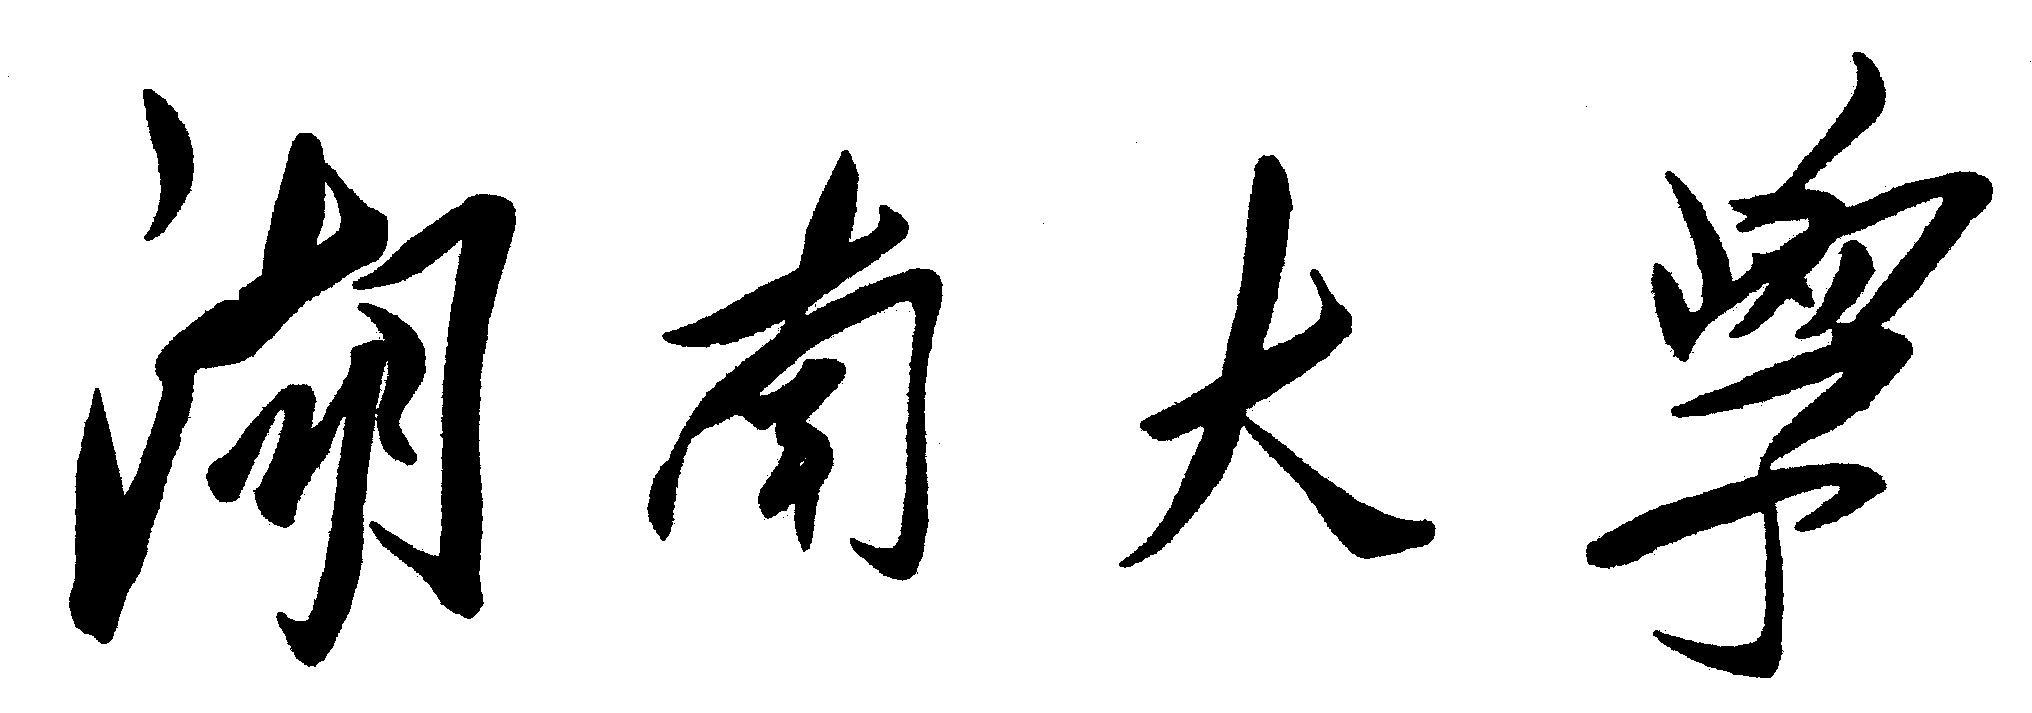
\includegraphics[width=8.01cm, height=2.58cm]{figures/hnu_logo.png}

    \makebox[0pt][c]{
        \raisebox{-0.5cm}[0pt][0pt]{
            \fontsize{26pt}{15pt}\selectfont \textbf{HUNAN UNIVERSITY}
        }
    }

    \makebox[0pt][c]{
        \raisebox{-2.5cm}[0pt][0pt]{
            \fontsize{45pt}{0}\selectfont {本科生毕业论文(设计)}
        }
    }

    \vspace{4.5cm}

    % 论文信息表格(无边框,带下划线)
    \renewcommand{\arraystretch}{1.3}
    \begin{tabular}{@{}r@{\hspace{0.5cm}}l@{}}
        {\fontsize{18pt}{15pt}\selectfont \textbf{论文(设计)题目:}} & {\fontsize{15pt}{15pt}\selectfont \underline{\makebox[9cm][l]{\thesisTitle}}} \\
        \addlinespace[1em]
        {\fontsize{14pt}{15pt}\selectfont 学~生~姓~名:} & {\fontsize{15pt}{15pt}\selectfont \underline{\makebox[9cm][l]{\studentName}}} \\
        \addlinespace[1em]
        {\fontsize{14pt}{15pt}\selectfont 学~生~学~号:} & {\fontsize{15pt}{15pt}\selectfont \underline{\makebox[9cm][l]{\studentID}}} \\
        \addlinespace[1em]
        {\fontsize{14pt}{15pt}\selectfont 专~业~班~级:} & {\fontsize{15pt}{15pt}\selectfont \underline{\makebox[9cm][l]{\studentMajor}}} \\
        \addlinespace[1em]
        {\fontsize{14pt}{15pt}\selectfont 学~院~名~称:} & {\fontsize{15pt}{15pt}\selectfont \underline{\makebox[9cm][l]{\studentAcademy}}} \\
        \addlinespace[1em]
        {\fontsize{14pt}{15pt}\selectfont 指~导~老~师:} & {\fontsize{15pt}{15pt}\selectfont \underline{\makebox[9cm][l]{\studentInstructor}}} \\
    \end{tabular}

    \vspace{1.5cm}
    {\fontsize{14pt}{15pt}\selectfont \thesisDate}

\end{titlepage}

% 原创性声明和版权授权书(封面之后,摘要之前)
\thispagestyle{empty}  % 不显示页眉页脚
\phantomsection\addcontentsline{toc}{chapter}{毕业论文（设计）原创性声明和毕业论文（设计）版权使用授权书}

\begin{center}
    {\sizeTwol \heiti 湖~南~大~学}
    
    \vspace{1cm}
    
    {\sizeTwol \heiti 毕业论文（设计）原创性声明}
\end{center}

\vspace{1.5cm}

本人郑重声明：所呈交的论文（设计）是本人在导师的指导下独立进行研究所取得的研究成果。除了文中特别加以标注引用的内容外，本论文不包含任何其他个人或集体已经发表或撰写的成果作品。对本文的研究做出重要贡献的个人和集体，均已在文中以明确方式标明。本人完全意识到本声明的法律后果由本人承担。

\vspace{0.5cm}

学生签名：\hspace{4.5cm}日期：~~~~~~~~年~~~~月~~~~日

\vspace{1cm}

\begin{center}
    {\sizeTwol \heiti 毕业论文（设计）版权使用授权书}
\end{center}

\vspace{1.25cm}

本毕业论文（设计）作者完全了解学校有关保留、使用论文（设计）的规定，同意学校保留并向国家有关部门或机构送交论文（设计）的复印件和电子版，允许论文（设计）被查阅和借阅。本人授权湖南大学可以将本论文（设计）的全部或部分内容编入有关数据库进行检索，可以采用影印、缩印或扫描等复制手段保存和汇编本论文（设计）。

本论文（设计）属于

\hspace{3.3cm}1、保\hspace{1em}密\hspace{0.5em}\raisebox{-1.5pt}{\framebox(12,12){}}，在\uline{\makebox[48pt][c]{}}年解密后适用本授权书。

\hspace{3.3cm}2、不保密\hspace{0.5em}\raisebox{-1.5pt}{\framebox(12,12){}}。

\hspace{3.3cm}（请在以上相应方框内打"√"）

\vspace{1cm}

学生签名：\hspace{4.5cm}日期：~~~~~~~~年~~~~月~~~~日

导师签名：\hspace{4.5cm}日期：~~~~~~~~年~~~~月~~~~日

\newpage

% 摘要和目录使用罗马数字页码
\pagenumbering{Roman}  % 大写的罗马数字
\setcounter{page}{1}

% 摘要
\begin{center}
    {\heiti\sizeThree 摘~~~~~~要}
\end{center}

\vspace{0.5cm}

\begin{center}
    {\heiti\sizeThreel \thesisTitle}
\end{center}

\vspace{0.5cm}

药物分子设计是药物研发的关键环节。传统方法依赖化学家经验和计算模拟,在处理高维化学空间搜索时效率较低、易陷入局部最优。近年来,大语言模型在自然语言处理领域取得突破,展现出强大的语义理解和生成能力,为分子设计带来新思路。

本研究提出LLM与进化算法结合的分子优化框架,用LLM的文本生成能力替代传统变异操作。通过设计自然语言提示词,引导LLM理解分子结构特征和优化目标,生成改进性质的新分子。该方法既利用LLM学到的化学知识,又保留进化算法的全局搜索优势。

我们构建了完整的LLM驱动优化系统,包括分子表示和属性预测、LLM交互接口、多种提示策略、种群管理等核心组件。设计了三种提示策略进行对比实验:基础优化提示、带示例的少样本学习提示、鼓励多样性的探索提示。实验结果表明,多样性鼓励策略在QED优化任务上效果最佳,能有效提升药物相似性分数并保持种群多样性,避免过早收敛。

此外,我们测试了LLM生成的随机性,发现适当提高温度参数能增加多样性,但过高会降低质量,需在探索和利用间平衡。多次独立运行显示方法具有良好稳定性和可重复性。

本研究为LLM在药物分子设计中的应用提供了可行方案,展示了NLP与计算化学交叉融合的可能性。未来可扩展到多目标优化、复杂属性预测及与其他生成模型结合。

\vspace{0.75cm}

\noindent {\heiti\sizeFour 关键词：}{\heiti\sizeFourl 大语言模型；进化算法；分子优化；药物设计；提示工程}

\newpage

\begin{center}
    {\bfseries\sizeThree Abstract}
\end{center}

\vspace{0.5cm}

\begin{center}
    {\bfseries\sizeThreel \thesisTitleENG}
\end{center}

\vspace{0.5cm}

Drug molecule design is crucial in drug development. Traditional methods rely on chemists' experience and computational simulations, facing low efficiency and local optima in high-dimensional chemical space search. Recently, large language models (LLMs) have achieved breakthroughs in natural language processing, demonstrating strong semantic understanding and generation capabilities, bringing new ideas to molecular design.

This study proposes a molecular optimization framework combining LLMs with evolutionary algorithms, using LLM's text generation to replace traditional mutation operations. By designing natural language prompts, we guide LLMs to understand molecular structures and optimization targets, generating improved molecules. This approach leverages chemical knowledge learned by LLMs while retaining evolutionary algorithms' global search advantages.

We constructed a complete LLM-driven optimization system, including molecular representation and property prediction, LLM interaction interface, multiple prompt strategies, and population management. Three prompt strategies were designed for comparative experiments: basic optimization, few-shot learning with examples, and diversity-encouraging exploration. Experimental results show that the diversity-encouraging strategy achieved the best performance in QED optimization, effectively improving drug-likeness scores while maintaining population diversity and avoiding premature convergence.

Additionally, we analyzed LLM generation randomness, finding that appropriately increasing temperature enhances diversity but excessive temperature reduces quality, requiring balance between exploration and exploitation. Multiple independent runs demonstrate good stability and reproducibility.

This research provides a feasible solution for applying LLMs in drug molecular design, showing the potential of NLP and computational chemistry integration. Future work can extend to multi-objective optimization, complex property prediction, and combination with other generative models.

\vspace{0.75cm}

\noindent {\bfseries\sizeFour Keywords: }{\bfseries\sizeFourl Large Language Model; Evolutionary Algorithm; Molecular Optimization; Drug Design; Prompt Engineering}

\newpage


% 目录（确保使用fancy样式显示页眉）
\pagestyle{fancy}
\tableofcontents
\newpage

% 正文从第1章开始使用阿拉伯数字页码
\pagenumbering{arabic}  % 阿拉伯数字
\setcounter{page}{1}

% 正文各章节
\chapter{绪论}

\section{研究背景与意义}

药物研发是一个周期很长、成本很高、风险也很大的过程,从最初的靶点发现到最后的临床试验,整个流程下来往往需要花费十几年甚至更长的时间,投入的资金也是以十亿美元来计算的\cite{di2019innovation}。在这个漫长的过程中,先导化合物的发现和优化是特别关键的一个环节,它直接决定了后续研发工作的成败。传统的药物分子设计主要依靠的是药物化学家的专业知识和经验积累,他们会根据对疾病机制的理解以及对受体结构的分析,来设计和合成具有潜在活性的化合物。不过这种方法存在一个很明显的问题,就是效率比较低,因为化学空间实在是太大了,据估计可能存在的类药分子数量达到了$10^{60}$这个级别\cite{bohacek1996art}，而人类能够实际合成和测试的分子数量只是其中很小的一部分。

为了解决这个问题,计算化学和计算机辅助药物设计(CADD)技术应运而生。这些技术通过建立数学模型和算法,能够在计算机上对大量的分子进行虚拟筛选和性质预测,从而缩小实验验证的范围,提高研发效率\cite{lyu2019ultra}。比如说定量构效关系(QSAR)方法,它就是通过统计分析已知的活性分子数据,建立起分子结构与生物活性之间的定量关系模型,然后用这个模型来预测新分子的活性\cite{muratov2020qsar}。还有分子对接技术,它可以模拟小分子配体与生物大分子受体之间的相互作用,评估结合的自由能,从而判断分子的潜在活性\cite{meng2011molecular}。这些计算方法在一定程度上缓解了传统实验方法的局限性,但是它们也面临着一些挑战。一方面,现有的预测模型的准确性还是有限的,特别是对于那些结构新颖的分子,预测结果往往不够可靠；另一方面,这些方法大多是基于局部搜索的策略,容易陷入局部最优解,难以在全局的化学空间中找到真正优秀的候选分子。

最近几年,人工智能技术的快速发展为药物研发带来了新的机遇。深度学习模型在图像识别、自然语言处理等领域取得了突破性的进展,也开始被应用到药物发现的各个环节中\cite{chen2018rise}。特别是在分子生成这个方向上,出现了很多基于深度学习的生成模型,比如变分自编码器(VAE)、生成对抗网络(GAN)、以及基于强化学习的方法等\cite{olivecrona2017molecular}。这些模型能够从已有的分子数据中学习化学空间的分布规律,然后生成具有特定性质的新分子结构。相比于传统的基于规则的方法,深度学习模型具有更强的表达能力和泛化能力,能够探索到更加广阔和复杂的化学空间。

在这些人工智能技术中,大语言模型(Large Language Model, LLM)的发展尤其引人注目。从GPT-3到GPT-4,再到各种开源的大模型如LLaMA\cite{touvron2023llama}、Qwen等,这些模型展现出了惊人的语言理解和生成能力\cite{achiam2023gpt}。它们不仅能够完成文本生成、机器翻译、问答系统等传统的自然语言处理任务,还能够在代码生成、逻辑推理、甚至是科学发现等方面发挥作用。大语言模型之所以能够做到这些,是因为它们在训练过程中接触到了海量的文本数据,从中学习到了丰富的世界知识和复杂的模式规律。这种强大的知识表示和推理能力,给很多领域都带来了启发,包括我们关注的药物分子设计领域。

把大语言模型应用到分子设计上,一个很自然的想法就是把分子的SMILES表示当成一种特殊的"语言"来处理。SMILES(Simplified Molecular Input Line Entry System)是一种用ASCII字符串来表示分子结构的记号系统,它能够把二维的分子图结构编码成一维的字符串,这样就能够利用自然语言处理的技术来进行处理和分析了\cite{weininger1988smiles}。事实上,已经有一些研究工作尝试用Transformer架构来学习SMILES序列的模式,并用于分子生成和性质预测\cite{schwaller2019molecular}。不过这些工作大多是专门训练一个针对分子的模型,而没有充分利用到预训练大语言模型已经在大规模通用语料上学到的知识和能力。

本研究就是要探索如何把现成的大语言模型直接应用到分子优化任务中,而不是重新训练一个专门的模型。我们的核心思路是用大语言模型的文本生成能力来替代传统进化算法中的变异操作,通过自然语言的提示词来引导模型理解优化的目标和要求,然后生成具有改进性质的新分子。这种方法有几个明显的优势：一是可以利用到大语言模型已经学到的丰富化学知识,不需要从头开始训练；二是通过自然语言的提示,可以灵活地调整优化的目标和约束条件,比传统的固定算子更加灵活；三是大语言模型本身具有很强的创造性,能够生成一些人类化学家可能想不到的新颖结构,有助于打破思维定式,发现新的化学空间区域。

从理论意义上来说,本研究探索了大语言模型在科学计算和工程设计领域的应用潜力,展示了自然语言处理技术与计算化学交叉融合的可能性。它为如何利用预训练模型的知识和能力来解决专业领域的复杂问题提供了一个具体的案例,对于推动人工智能技术在科学研究中的应用具有积极的意义。从实际应用的角度来看,如果能够证明这种方法是有效的,那么它就可以作为一个辅助工具,帮助药物化学家更快地找到有潜力的候选分子,缩短药物研发的周期,降低研发的成本。虽然目前这个方法还处于初步探索的阶段,距离真正的工业应用还有一定的距离,但是它所体现的思路和方向是值得深入研究和发展的。

\section{国内外研究现状}

在大语言模型应用于分子设计这个方向上,国内外的研究者都已经开展了一些相关的探索工作。从国外的研究来看,Molecular Transformer是最早引起关注的工作之一。Schwaller等人提出用Transformer模型来预测化学反应的产物,他们把反应物和试剂的SMILES作为输入,产物的SMILES作为输出,通过大量的反应数据进行训练,使得模型能够学习到化学反应的规律\cite{schwaller2019molecular}。这个模型在多个基准测试数据集上都取得了很好的效果,证明了Transformer架构在处理化学序列数据方面的有效性。在此基础上,后续的研究者又提出了各种改进的版本,比如加入注意力机制的解释性分析、引入反应条件的信息、以及扩展到逆合成分析等任务。

除了反应预测,直接用大语言模型来生成分子也是一个活跃的研究方向。ChemBERTa是一个专门为化学领域设计的预训练语言模型,它在数百万个分子SMILES数据上进行了掩码语言模型的预训练,学习到了分子的语法和语义特征\cite{chithrananda2020chemberta}。研究表明,经过预训练的ChemBERTa在下游的分子性质预测任务上,只需要少量的标注数据就能达到很好的性能,这体现了预训练-微调范式在化学领域的适用性。类似的工作还有MoLFormer,它采用了不同的预训练策略和模型架构,也在多个基准测试中表现优异\cite{ross2022molformer}。这些工作说明,针对化学领域进行专门的预训练,确实能够提升模型在相关任务上的表现。

不过上述这些工作都是要重新训练或者微调一个专门的模型,这需要大量的计算资源和标注数据。与之不同的是,有一些研究者开始探索如何直接使用通用的大语言模型来完成化学任务。比如Galactica模型,它是Meta公司推出的一个面向科学知识的大型语言模型,在训练数据中包含了大量的科学文献、教科书、以及数据库信息\cite{taylor2022galactica}。研究发现,Galactica能够在不进行专门微调的情况下,完成分子性质预测、反应预测、甚至是论文写作等任务,展现出了很强的零样本和小样本学习能力。这说明通用的大语言模型确实已经学到了一定的化学知识,可以直接应用于一些化学相关的任务。

在国内,相关的研究起步稍微晚一些,但是发展速度很快。清华大学、北京大学、中国科学院等机构的研究团队都在这个方向上开展了工作。比如清华大学的团队提出了一种结合知识图谱和大语言模型的分子生成方法,通过知识图谱提供结构化的化学知识,大语言模型负责生成和推理,两者互补,提高了生成分子的质量和多样性\cite{wang2024knowledge}。北京大学的团队则专注于多目标分子优化,他们设计了复杂的提示词策略,让大语言模型能够同时考虑多个药物属性指标,生成综合性能更好的分子\cite{liu2024multi}。这些工作都体现了国内研究者在这个前沿领域的积极探索和创新精神。

在进化算法与机器学习结合方面,也有很多相关的研究。传统的进化算法包括遗传算法、进化策略、粒子群优化等,它们在组合优化、参数调优等问题上有着广泛的应用\cite{holland1992genetic,eiben2015introduction}。近年来,研究者开始尝试用机器学习模型来增强进化算法的各个组件,比如用神经网络来预测个体的适应度,减少昂贵的评估次数；用强化学习来选择变异算子,提高搜索的效率；用生成模型来初始化种群,提供更好的起点等\cite{karafotias2014parameter}。这些工作被称为"神经进化"或者"学习型进化算法",它们的核心思想是利用机器学习模型的泛化能力和预测能力,来弥补传统进化算法盲目搜索的不足。

本研究提出的方法可以看作是神经进化的一个具体实例,不过我们用大语言模型替代了传统的变异算子,这是一个比较新颖的尝试。与之前的工作相比,我们的方法有几个特点：一是完全依赖于预训练的大语言模型,不需要额外的训练或微调；二是通过自然语言提示来实现灵活的优化目标控制；三是保留了进化算法的种群机制和选择压力,确保搜索的方向性和有效性。这些特点使得我们的方法在实现简单性和应用灵活性方面具有一定的优势。

\section{研究内容与目标}

基于以上的研究背景和现状分析,本研究的主要目标是探索和验证大语言模型在分子进化优化中的应用可行性。具体来说,我们要回答以下几个核心问题：第一,大语言模型是否能够理解分子的SMILES表示,并根据提示生成化学上有效且具有改进性质的新分子；第二,不同的提示词策略对生成结果有什么样的影响,哪种策略更有效；第三,把大语言模型集成到进化算法框架中,能否实现有效的分子优化,其性能 compared to 传统方法如何；第四,大语言模型生成的随机性对优化过程有什么影响,如何控制和利用这种随机性。

围绕这些问题,本研究的具体内容包括以下几个方面：

一是构建一个完整的LLM驱动的分子进化优化系统。这个系统需要整合多个功能模块,包括分子表示和验证模块,用来处理和验证SMILES字符串的化学有效性；属性预测模块,用来计算分子的各种药物属性指标,如QED、LogP、分子量等；大语言模型交互接口,用来调用本地的Ollama服务,发送提示并接收生成的结果；提示词模板设计,根据不同的优化策略设计合适的提示词格式和内容；种群管理模块,负责维护分子种群,执行选择、更新等操作；以及结果分析和可视化模块,用来记录实验数据和生成图表。

二是设计和实现多种提示词策略。我们计划设计三种不同层次的提示策略,从简单到复杂,逐步增加提示的信息量和指导性。第一种是基础优化提示,只包含当前分子的SMILES、目标属性名称、以及当前的分数,要求模型生成改进的分子。第二种是带示例的少样本学习提示,在基础提示的基础上,增加几个成功优化的例子,让模型能够通过类比学习来理解优化的策略。第三种是鼓励多样性的探索提示,除了基本的优化要求外,还会告诉模型近期已经生成过的分子,要求它避免重复,尝试新的化学结构。通过对比这三种策略的效果,我们可以了解提示信息对模型生成行为的影响规律。

三是进行系统的实验验证和性能评估。我们会选择QED(定量估计药物相似性)作为主要的优化目标,因为它是一个综合性的指标,能够反映分子的药物开发潜力。实验会分为几个部分：首先是对比三种提示策略的优化效果,看哪种策略能够更快地提升QED分数；其次是分析种群的多样性变化,检查是否存在过早收敛的问题；然后是测试大语言模型生成的随机性,通过调整温度参数和控制多次运行,来评估结果的稳定性和可重复性；最后是与基线方法进行对比,虽然我们没有实现传统的进化算法作为对照,但是可以通过文献中的数据来进行定性的比较分析。

四是总结和提炼研究的发现和启示。在实验的基础上,我们会分析大语言模型在分子优化任务中的优势和局限性,探讨可能的改进方向和应用前景。同时也会反思研究过程中遇到的问题和挑战,为后续的研究工作提供参考和建议。

\section{论文组织结构}

本论文的其余部分组织如下：第二章介绍相关的理论基础和技术背景,包括分子表示方法、药物属性预测、进化算法的基本原理、以及大语言模型的工作机制等,为后续的方法设计和实验分析奠定理论基础。第三章详细阐述我们提出的LLM驱动的分子进化优化方法,包括系统的整体架构、各个模块的设计和实现、提示词策略的设计思路、以及关键的算法流程等。第四章呈现实验的结果和分析,包括实验设置、对比实验的结果、多样性分析、随机性测试、以及结果讨论等。第五章总结全文的主要工作和贡献,指出研究的不足之处,并对未来的研究方向进行展望。

\include{chapter2_related_work}
\chapter{基于LLM的分子进化优化方法}

\section{系统整体架构}

本研究提出的LLM驱动的分子进化优化系统,是一个把大语言模型的生成能力和进化算法的搜索机制有机结合起来的框架。系统的核心思想是用自然语言提示来引导大语言模型理解分子优化的目标,然后让模型生成具有改进性质的新分子结构,再通过进化算法的选择和更新机制来维持种群的质量和多样性。整个系统由六个主要的模块组成,分别是分子表示与验证模块、属性预测模块、大语言模型交互接口、提示词模板设计模块、种群管理模块、以及结果分析与可视化模块。这些模块相互配合,共同完成分子的迭代优化过程。

近年来,将大语言模型用作进化优化器的研究逐渐兴起。Liu等人\cite{liu2023llm}首次系统地提出了"Large Language Models as Evolutionary Optimizers"的概念,证明了LLM可以在不需要专门训练的情况下执行优化任务。Reinhart和Statt\cite{reinhart2024llm}进一步将这一方法应用到序列定义的大分子设计中,展示了LLM在化学领域的潜力。Brahmachary等人\cite{brahmachary2024llm}开发了基于LLM的进化优化器,并验证了其在多个基准测试中的有效性。Wang等人\cite{wang2025multi}则探索了多智能体LLM系统在进化优化中的应用,提出了MAEF框架。这些工作为本研究提供了重要的理论基础和实践参考。

从数据流的角度来看,系统的工作流程是这样的：首先,从初始的分子池中选择一定数量的分子,构成初始种群,每个分子用SMILES字符串表示,并计算其药物属性作为适应度；然后,在每一代的进化中,根据选择策略从当前种群中选择出优秀的个体作为父代；接着,对每个父代分子,根据其SMILES和当前的属性值,构建合适的提示词,发送给大语言模型,请求生成改进的分子；大语言模型返回生成的SMILES字符串后,系统进行解析和验证,过滤掉无效的分子,并计算新分子的属性值；之后,把新生成的子代分子加入到种群中,同时移除一些较差的个体,保持种群规模不变；最后,记录当前代的统计信息,包括最佳适应度、平均适应度、种群多样性等,用于后续的分析和可视化。这个过程会重复进行,直到达到预设的最大代数或者满足其他终止条件。

系统的架构设计遵循了模块化和可扩展性的原则。每个模块都有清晰的接口和职责,可以独立地进行测试和改进。比如,如果想更换不同的大语言模型,只需要修改LLMClient模块的配置,不需要改动其他部分；如果想尝试新的提示策略,只需要在PromptTemplates模块中添加新的模板,就可以在实验中直接使用；如果想优化其他的药物属性,只需要在PropertyPredictor模块中添加相应的计算函数,并在初始化时指定即可。这种设计使得系统具有很强的灵活性,能够适应不同的研究需求和应用场景。

在技术实现上,我们使用了Python作为主要的编程语言,因为它有丰富的科学计算和化学信息学库支持。具体来说,我们使用了RDKit库来进行分子的处理和属性计算,RDKit是化学信息学领域最流行的开源工具包之一,提供了完整的分子表示、转换、验证、以及性质预测功能；我们使用了NumPy和Pandas库来进行数值计算和数据处理,这两个库是Python科学计算的基础设施,提供了高效的数组操作和数据框处理功能；我们使用了Requests库来调用Ollama的API接口,实现与大语言模型的交互；我们还使用了Matplotlib库来生成可视化的图表,帮助分析实验结果。所有的代码都组织成了清晰的模块结构,便于理解和维护。

\section{分子表示与验证模块}

分子表示与验证模块是整个系统的基础,它负责处理分子的SMILES字符串,确保所有参与优化的分子都是化学上有效的。这个模块的核心是MoleculeUtils类,它封装了RDKit库的相关功能,提供了一系列实用的工具函数。

SMILES标准化的处理是这个模块的一个重要功能。如前面提到的,同一个分子可能有多种不同的SMILES表示,这被称为SMILES异构性。比如说,苯环可以表示为"c1ccccc1",也可以表示为"c1cccc c1"(中间有空格,虽然这不是合法的SMILES,但是说明了顺序可以不同),甚至可以从不同的原子开始遍历,得到不同的字符串。这种异构性会给分子的比较、去重、以及追踪带来困难。为了解决这个问题,我们对每个输入的SMILES都进行标准化处理。标准化的过程是：先用RDKit把SMILES解析成分子对象,如果解析失败,说明这个SMILES是无效的,直接丢弃；如果解析成功,再用RDKit的Canonical SMILES功能重新生成标准的SMILES字符串。Canonical SMILES是根据一套确定的规则生成的,保证同一个分子只会得到一个唯一的表示。通过这种方式,我们可以有效地消除SMILES异构性带来的问题。

分子有效性验证是另一个关键的功能。大语言模型生成的SMILES字符串不一定都是化学上有效的,可能会存在语法错误(如括号不匹配、环标记错误)、价态不合理(如碳原子连接了5个键)、或者结构不稳定等问题。对于无效的分子,我们需要在早期就过滤掉,避免它们进入后续的优化流程。我们的验证策略是分层次的：第一层是语法检查,即尝试用RDKit解析SMILES,如果解析失败,说明语法有问题；第二层是化学合理性检查,即检查分子的原子价态是否合理,是否有不可能的结构；第三层是可选的额外检查,比如检查分子量是否在合理范围内,是否有有毒的子结构等。只有通过所有检查的分子才会被认为是有效的,才能进入种群。

除了标准化和验证,MoleculeUtils类还提供了一些辅助功能,比如从文件中读取SMILES列表、过滤无效SMILES、计算分子的基本描述符等。这些功能虽然在核心的优化流程中不是必需的,但是在数据预处理和结果分析时会用到,提高了代码的复用性和可维护性。

在实际的使用中,我们会发现大语言模型生成的SMILES有效率并不是100\%,有时候会有20\%-30\%甚至更高的无效率。这主要是因为大语言模型虽然学到了大量的化学知识,但是它本质上还是一个统计模型,是基于概率来生成下一个字符的,并不能完全保证生成的结果是化学上合理的。为了提高有效率,一方面我们可以通过改进提示词,给模型更明确的指导和约束；另一方面我们可以在后处理阶段进行严格的验证和过滤,只保留有效的分子。在我们的实验中,通过这两种方法的结合,最终的有效率可以控制在可接受的范围内,不会对整体的优化效果产生太大的影响。

\section{属性预测模块}

属性预测模块负责计算分子的各种药物相关属性,这些属性值是评估分子质量和指导优化方向的关键依据。我们的PropertyPredictor类提供了一个统一的接口来预测不同的属性,目前主要支持QED、LogP、分子量、氢键供体/受体数量等常用指标。

QED属性的计算是我们最关注的,因为它是本研究中主要的优化目标。QED的计算公式比较复杂,它基于八个分子描述符,每个描述符都有一个理想的范围和一个对应的得分函数。得分函数通常是钟形曲线或者S形曲线,当描述符的值在理想范围内时,得分接近1；偏离理想范围时,得分逐渐降低。最终的QED值是这八个得分的几何平均值,这样能够保证任何一个描述符的严重偏离都会显著降低总的QED分数。RDKit库提供了rdkit.Chem.QED.qed()函数来计算QED,这个函数的实现是基于原始论文的公式,准确性是有保证的。在我们的系统中,每次生成新的分子后,都会立即调用这个函数来计算QED值,作为该分子的适应度。

除了QED,我们还实现了其他属性的预测函数,虽然在本研究中没有作为优化目标,但是它们可以作为辅助信息来帮助分析分子的特性。比如LogP,我们用rdkit.Chem.Crippen.MolLogP()函数来计算,它基于原子贡献的方法,把分子分解成各种原子类型和键类型,每种类型有一个预定义的贡献值,最后把所有贡献值加起来得到LogP。分子量是通过累加所有原子的原子量得到的,RDKit提供了准确的原子量数据。氢键供体和受体的计数是通过分析分子中的官能团来实现的,比如羟基(-OH)、氨基(-NH2)等是氢键供体,羰基(C=O)、醚氧(-O-)等是氢键受体。

PropertyPredictor类的设计考虑了扩展性。如果将来需要支持更多的属性,只需要在类中添加新的预测方法,并在predict()函数中添加相应的分支即可。另外,我们也考虑了性能优化的可能性。目前的实现是每次调用都重新计算属性值,对于大规模的数据集可能会比较慢。一种优化的方案是引入缓存机制,把已经计算过的分子的属性值存储起来,下次遇到相同的分子时直接从缓存中读取,避免重复计算。另一种方案是用机器学习模型来替代传统的计算方法,训练一个回归模型来预测属性值,这样可以大大提高计算速度,特别是对于复杂的属性如毒性、生物活性等,机器学习模型可能比经验规则更准确。

在异常处理方面,PropertyPredictor类也做了充分的考虑。如果输入的SMILES无效,或者计算过程中出现错误,预测函数会返回-1作为错误标志,调用方可以根据这个标志来判断计算是否成功,并采取相应的措施,比如丢弃这个分子或者重试。这种健壮的设计保证了系统在面对异常情况时不会崩溃,能够稳定地运行。

\section{大语言模型交互接口}

大语言模型交互接口是系统与外部LLM服务通信的桥梁,它负责发送提示词、接收生成的结果、以及处理可能的错误。我们的LLMClient类封装了与Ollama API的交互逻辑,提供了一个简洁易用的接口。

Ollama是一个本地部署的大语言模型运行工具,它支持多种开源模型,包括LLaMA、Qwen、Mistral等。Ollama提供了一个RESTful API,我们可以通过HTTP请求来调用模型的生成功能。API的端点是http://localhost:11434/api/generate,请求的参数包括模型名称(model)、提示词(prompt)、是否流式输出(stream)、以及生成选项(options)等。生成选项中可以设置温度(temperature)、Top-k、Top-p等采样参数,用来控制生成的随机性和多样性。

LLMClient类的generate()方法是核心的功能函数。它接收一个提示词字符串和生成数量n作为参数,然后构造HTTP POST请求,发送给Ollama API。请求成功后,API会返回一个JSON格式的响应,其中包含生成的文本(response字段)。我们从响应中提取出生成的文本,然后调用\_parse\_smiles\_from\_text()方法来解析出SMILES字符串。解析的过程是按行分割文本,去除序号标记(如"1."、"2)"等),然后对每一行进行简单的验证,检查长度是否在合理范围内,是否包含字母字符等。通过验证的行会被当作SMILES字符串返回。

在错误处理方面,LLMClient类也做了周全的考虑。如果Ollama服务没有启动,或者网络连接失败,requests库会抛出ConnectionError异常,我们会捕获这个异常并给出友好的提示信息,告诉用户需要先启动Ollama服务。如果API返回的状态码不是200,说明请求失败了,我们会打印出状态码,方便调试。如果解析后的SMILES列表为空,可能是模型没有按照要求生成SMILES,或者生成的格式不符合预期,这种情况下我们会返回空列表,调用方可以根据情况决定是否重试。

为了提高效率,我们在generate()方法中添加了批量生成的支持。通过设置n参数,可以一次性请求生成多个分子,而不是多次调用API。这样能够减少网络开销和等待时间,提高整体的吞吐量。不过需要注意的是,Ollama API的generate端点一次只能生成一个序列,所以所谓的"批量生成"实际上是在提示词中要求模型生成多个SMILES,然后在后处理时解析出来。这种方法的效果取决于模型的能力,有时候模型可能不会严格按照要求生成指定数量的SMILES,这时候就需要在解析时做灵活的处理。

在模型选择上,我们默认使用qwen2.5:7b模型,这是阿里巴巴通义实验室开发的开源大语言模型,有70亿个参数。这个模型在中文和英文的理解和生成上都有不错的表现,而且在消费级的GPU上就可以运行,非常适合学术研究和小规模的应用。当然,LLMClient类的设计是通用的,可以通过修改model\_name参数来使用其他模型,比如llama3.2:3b、mistral:7b等,只要Ollama支持就行。这种灵活性使得我们可以方便地比较不同模型的性能,选择最适合任务的模型。

温度参数的设置对生成结果有很大的影响。温度越高,生成的结果越多样化,但是也越不可控,可能会出现更多无效的SMILES；温度越低,生成的结果越确定性高,质量可能更好,但是多样性不足,容易陷入局部最优。在我们的实验中,我们默认设置温度为0.8,这是一个折中的选择,既保证了一定的多样性,又不至于让质量下降太多。在第四章的随机性测试中,我们会系统地研究温度参数对生成结果的影响,并给出推荐的取值范围。

\section{提示词模板设计}

提示词模板设计是本研究的一个核心创新点,也是影响优化效果的关键因素。提示词的作用是把分子优化的任务用自然语言的形式表达出来,让大语言模型能够理解我们的意图,并按照要求生成改进的分子。好的提示词应该清晰明确地传达以下信息：当前的分子是什么(SMILES)、需要优化的属性是什么、当前的属性值是多少、生成的要求是什么(如数量、格式、约束条件)等。

我们设计了三种不同层次的提示策略,从简单到复杂,逐步增加提示的信息量和指导性。这三种策略分别是基础优化提示(Basic Optimization)、带示例的少样本学习提示(With Examples)、以及鼓励多样性的探索提示(Diversity Encouraging)。下面我们来详细介绍每种策略的设计思路和具体实现。

基础优化提示是最简单的策略,它只包含了完成任务所需的最基本信息。提示词的格式大致是："你是一个专业的药物化学家,擅长设计具有特定性质的药物分子。任务：优化分子的[属性名]分数,使其更高。当前分子SMILES：[SMILES]。当前[属性名]分数：[分数]。要求：1. 生成的分子必须是化学上有效的SMILES格式；2. 保持分子的核心骨架；3. 通过修改官能团或侧链来优化[属性名]；4. 每行输出一个SMILES,不要有其他解释。请生成3个改进后的分子SMILES："。这个提示词的优点是简洁明了,不会给模型太多的干扰信息；缺点是缺乏具体的指导,模型可能需要依靠自己的判断来决定如何优化,这可能导致生成的结果不够理想。

带示例的少样本学习提示在基础提示的基础上,增加了一两个成功优化的例子。这些例子展示了从输入分子到输出分子的转变过程,以及优化的策略。比如："参考以下成功优化的例子：例子1：输入：CC(=O)Oc1ccccc1C(=O)O (QED=0.55),输出：CC(=O)Oc1ccc(Cl)cc1C(=O)O (QED=0.78),改进策略：在苯环上添加氯原子,增加亲脂性。现在,请优化以下分子：..."。这种做法利用了大语言模型的上下文学习能力,让模型能够通过类比来理解优化的思路。研究表明,少样本学习能够显著提升大语言模型在特定任务上的表现,因为它给模型提供了具体的参考,减少了不确定性。不过,示例的选择也很重要,如果示例不具有代表性,或者与当前任务差异太大,可能会起到反作用。

鼓励多样性的探索提示是最高级的策略,它不仅要求模型优化属性,还要求模型保持多样性,避免生成与近期分子相似的结构。提示词中会包含近期已生成的分子列表(通常是最近5个),并明确要求"尝试与近期分子不同的化学结构"、"探索新的官能团和骨架"等。这种策略的目的是防止种群过早收敛,保持搜索的广度和深度。在进化算法中,多样性是一个非常重要的指标,如果种群的多样性太低,所有的个体都聚集在搜索空间的某个小区域,那么就很难找到更好的解。通过鼓励多样性,我们可以让模型主动探索新的化学空间区域,增加找到全局最优解的可能性。当然,这种策略也有风险,就是可能会牺牲一些优化的效率,因为模型需要在多样性和质量之间做权衡。

除了这三种基本策略,我们还设计了多目标优化提示(Multi-objective Optimization),用于同时优化多个属性的场景。这种提示词会列出所有的优化目标,包括属性名称、当前值、以及优化的方向(提高还是降低),并要求模型尽可能同时改善多个性质。如果难以兼顾,可以优先保证最重要的性质。多目标优化是药物设计中的一个常见需求,因为一个好的药物候选物需要在多个方面都达到要求,而不仅仅是某一个属性特别突出。虽然在本研究中我们没有重点实验多目标优化,但是这个功能已经实现,可以在后续的工作中进一步探索。

提示词的设计是一个迭代的过程,需要根据实验的结果不断地调整和改进。我们发现,不同的模型可能对提示词的敏感度不同,有些模型需要更详细的说明,有些模型则能够从简洁的提示中理解意图。另外,提示词的长度也是一个需要考虑的因素,过长的提示词可能会超出模型的上下文窗口,或者让模型难以抓住重点；过短的提示词又可能信息不足,导致生成的结果不符合要求。在我们的实验中,我们通过多次试错,找到了一个平衡点,使得提示词既能够提供足够的信息,又不会过于冗长。

\section{种群管理与选择机制}

种群管理模块负责维护分子的集合,执行选择、更新、以及统计记录等操作。我们的Population类实现了完整的种群管理功能,包括个体的存储、适应度的计算、父代的选择、种群的更新、以及历史的记录等。

个体(Individual)是种群的基本单元,每个个体代表一个分子。Individual类包含了以下属性：smiles(分子的SMILES字符串)、properties(属性字典,存储各种药物属性的值)、fitness(综合适应度,用于比较个体的优劣)、generation(所属的世代,记录这个个体是在哪一代产生的)、parents(父代SMILES列表,用于追溯谱系)。在这些属性中,fitness是最重要的,它决定了个体在选择过程中的被选中概率。fitness的计算是通过calculate\_fitness()方法完成的,它会根据各个属性的值和权重,计算一个加权平均分。默认情况下,所有属性的权重相等,但是也可以通过weights参数来自定义权重,实现对不同属性的侧重。

种群(Population)的初始化是从一个SMILES列表中随机采样一定数量的分子,然后为每个分子计算属性值和适应度。采样的策略是：如果SMILES列表的数量大于种群规模,就随机抽取种群规模数量的分子；如果SMILES列表的数量小于种群规模,就先全部使用,然后重复随机选择,直到达到种群规模。这种策略保证了初始种群的多样性,同时也确保了种群规模的固定。初始化完成后,会调用\_update\_archive()方法来更新历史最优档案,把当前最优的个体保存起来,用于后续的分析和比较。

父代选择是进化算法中的一个关键步骤,它决定了哪些个体有机会产生后代。我们实现了三种选择方法：锦标赛选择(Tournament Selection)、轮盘赌选择(Roulette Wheel Selection)、以及Top-K选择。锦标赛选择是随机选取k个个体(称为锦标赛大小),从中选择适应度最高的那个作为父代。这个过程的优点是选择压力可控,通过调整k的大小,可以调节选择的强度；k越大,选择压力越大,优秀个体被选中的概率越高。轮盘赌选择是按照适应度的比例来分配选择概率,适应度越高的个体,被选中的概率越大。这种方法的优点是直观易懂,符合"优胜劣汰"的直觉；缺点是对适应度的绝对值敏感,如果有个别个体的适应度特别高,可能会垄断选择,导致多样性下降。Top-K选择是直接选择适应度最高的k个个体,这是一种确定性的选择方法,选择压力最大,但是多样性最差。在我们的实验中,默认使用锦标赛选择,因为它在实践中的表现比较均衡。

种群更新是把新生成的子代个体加入到种群中,同时移除一些旧的个体。我们实现了两种更新策略：稳态更新(Steady-State Update)和世代更新(Generational Update)。稳态更新的策略是把当前种群和新个体合并,然后按适应度从高到低排序,取前N个(N是种群规模)作为新的种群。这种方法的优点是保留了最优秀的个体,不管它们是来自当前代还是新一代,进化的过程比较平稳。世代更新的策略是完全用新个体替换旧个体,但是保留当前最优的个体(精英策略)。这种方法的优点是进化速度快,能够快速响应新的变化；缺点是可能会丢失一些有价值的历史信息。在我们的实验中,默认使用稳态更新,因为它能够更好地保持种群的稳定性和连续性。

除了选择和更新,Population类还提供了其他有用的功能。get\_best()方法可以获取适应度最高的N个个体,用于结果的展示和分析。get\_diversity()方法计算种群的多样性,定义为不同SMILES的数量占总个体数的比例。多样性的值在0到1之间,1表示所有个体都不相同,0表示所有个体都相同。多样性是监控进化过程的重要指标,如果多样性持续下降,说明种群可能在过早收敛,需要采取措施(如增加变异率、引入新的个体等)来恢复多样性。to\_dataframe()方法把种群转换成Pandas DataFrame,方便导出到CSV文件或者进行进一步的分析。save()方法可以把种群保存到文件中,用于后续的加载和继续优化。

历史记录(history)功能是用来追踪进化过程的。每一代结束后,\_record\_history()方法会记录当前的统计信息,包括世代号、最佳适应度、平均适应度、适应度标准差、种群大小、以及各个属性的最佳值和平均值等。这些信息可以用来绘制收敛曲线,分析优化的进展,诊断可能出现的问题。比如,如果最佳适应度连续多代没有提升,说明可能已经达到了局部最优,需要考虑改变策略；如果平均适应度和最佳适应度的差距很大,说明种群的分布不均匀,可能存在一些特别优秀的个体和很多较差的个体。

\section{算法流程与实现细节}

综合上述各个模块,我们得到了完整的LLM驱动的分子进化优化算法。算法的整体流程可以用以下的伪代码来描述：

初始化种群：从SMILES池中随机选择N个分子,计算它们的属性值和适应度；
记录初始统计信息；
对于每一代(gen = 1 to max\_generations)：
  选择父代：根据选择方法,从当前种群中选择K个父代个体；
  生成子代：对于每个父代：
    构建提示词：根据提示策略,生成包含父代SMILES和优化目标的提示；
    调用LLM：发送提示给大语言模型,请求生成M个新分子；
    解析结果：从LLM的响应中提取SMILES字符串；
    验证分子：对每个SMILES进行标准化和有效性检查；
    计算属性：对有效的分子,计算其属性值和适应度；
    记录成功案例：如果子代的属性优于父代,把这个案例加入示例库；
  更新种群：把子代个体加入到种群中,移除最差的个体,保持种群规模为N；
  记录统计信息：计算当前代的最佳适应度、平均适应度、多样性等；
  输出进度：每隔一定代数,打印当前的最佳分子和属性值；
结束循环；
保存结果：把最终的种群和统计信息保存到文件中；
返回统计数据的DataFrame。

在这个流程中,有几个关键的实现细节需要注意。一是提示词的构建,它需要根据当前的提示策略来选择不同的模板,并填充相应的信息。我们的\_build\_prompt()方法实现了这个逻辑,它会根据self.prompt\_strategy的值,调用PromptTemplates类中对应的静态方法,生成最终的提示词字符串。二是子代的生成和验证,这是一个耗时的过程,因为需要调用LLM API,并且对每个生成的分子进行属性计算。为了提高效率,我们采用了批量生成的方式,一次请求生成多个分子,然后用并行或者串行的方式进行验证和计算。三是去重的处理,为了避免种群中出现重复的分子,我们在\_generate\_offspring()方法中对子代进行了去重,使用一个集合(seen\_smiles)来记录已经出现过的SMILES,只保留第一次出现的个体。四是示例库的维护,当子代的属性优于父代时,我们会把这个成功的案例记录下来,包括输入分子、输出分子、以及改进的幅度。这些案例可以用于后续的分析和可视化,也可以用于增强提示词(如在带示例的提示中使用)。

在代码的组织上,我们把核心的优化逻辑封装在LLMEvolutionaryOptimizer类中,这个类整合了所有的模块,提供了统一的接口。用户可以通过设置参数来控制优化的各个方面,如property\_name(优化目标属性)、population\_size(种群规模)、llm\_model(使用的LLM模型)、prompt\_strategy(提示策略)、selection\_method(选择方法)、temperature(生成温度)、children\_per\_parent(每个父代生成的子代数)、survival\_rate(存活率,决定每代选择多少个父代)、max\_generations(最大代数)、output\_dir(输出目录)等。这种参数化的设计使得实验的配置非常灵活,可以通过修改参数来快速尝试不同的设置。

run()方法是执行完整优化流程的入口函数。它会打印开始的配置信息,然后进入主循环,逐代执行优化。在每一代结束后,如果代数是指定的间隔(如每5代)或者是第一代,会打印当前的最佳分子信息,让用户能够实时了解优化的进展。优化完成后,会调用save\_results()方法保存结果,并返回统计数据的DataFrame,方便后续的分析。

总的来说,我们的实现充分考虑了实用性、可扩展性、和易用性。代码结构清晰,注释充分,便于理解和修改。通过合理的抽象和封装,各个模块之间的耦合度很低,可以独立地进行测试和改进。这种设计不仅满足了本研究的需求,也为后续的工作奠定了良好的基础。

\chapter{实验与结果分析}
\vspace{7pt}


\section{实验设置}

为了全面评估我们提出的LLM驱动的分子进化优化方法的性能,我们设计了一系列的实验,包括不同提示策略的对比实验、种群多样性分析、随机性测试等。本节将详细介绍实验的设置,包括数据集的选择、参数的配置、评价指标的定义、以及实验环境的说明。

在数据集方面,我们没有使用大规模的分子数据库,而是采用了一个小规模的测试集,包含了三个常见的药物分子:阿司匹林(Aspirin)、咖啡因(Caffeine)、以及布洛芬(Ibuprofen)。这三个分子的SMILES编码如下所示:

% \begin{figure}[htbp]
% \centering
% \begin{minipage}{0.3\linewidth}
% \centering
% \setchemfig{atom sep=2em}
% \chemfig{*6(-=-=-(-C(=[2]O)-[6]OH)=)}
% \caption*{阿司匹林}
% \end{minipage}
% \hfill
% \begin{minipage}{0.3\linewidth}
% \centering
% \setchemfig{atom sep=2em}
% \chemfig{N_1-[:30]C(=[2]N-[:330]C(=[6]N_1)-[:-30]N(-[:30]CH_3)-[:330]C(=[6]O))}
% \caption*{咖啡因}
% \end{minipage}
% \hfill
% \begin{minipage}{0.3\linewidth}
% \centering
% \setchemfig{atom sep=2em}
% \chemfig{*6(=-(-CH_2-CH(-[6]CH_3)(-[2]CH_3))=-=(-CH(-[6]CH_3)-C(=[2]O)-[6]OH)-=)}
% \caption*{布洛芬}
% \end{minipage}
% \end{figure}

SMILES(Simplified Molecular Input Line Entry System)是一种用字符串表示分子化学结构的记号系统。对应的SMILES编码为：
\begin{itemize}
\item 阿司匹林：\texttt{CC(=O)Oc1ccccc1C(=O)O}
\item 咖啡因：\texttt{CN1C=NC2=C1C(=O)N(C(=O)N2C)C}
\item 布洛芬：\texttt{CC(C)CC1=CC=C(C=C1)C(C)C(=O)O}
\end{itemize}

SMILES编码规则很简单：字母表示原子(C=碳,O=氧,N=氮),符号表示化学键(=双键,\#三键),数字标记环结构,括号表示支链。比如乙醇的SMILES是\texttt{CCO},表示两个碳原子和一个氧原子连接。这种编码方式能够把二维的分子结构图转换成一维文本,非常适合大语言模型处理。

选择这三个分子的原因是它们都是广泛使用的非处方药,具有代表性的化学结构,而且它们的QED分数处于中等水平(大约在0.5到0.6之间),有优化的空间。在实验中,我们把这三个分子的SMILES重复多次,构成一个初始池,然后从中随机采样来初始化种群。这种设置虽然简单,但是足以验证方法的有效性,同时也便于快速完成实验,适合本科毕业设计的规模。

在参数配置方面,我们进行了多次试验,最终确定了一组比较合理的默认参数。种群规模(population\_size)设置为20,这是一个适中的大小,既能够保持一定的多样性,又不会导致计算开销过大。每个父代生成的子代数(children\_per\_parent)设置为3,这意味着每一代总共会生成大约60个子代(20个父代 $\times$ 3个子代),然后通过选择保留最优秀的20个。存活率(survival\_rate)设置为0.3,即每代选择6个父代(20 $\times$ 0.3 = 6)来产生子代,这个比例能够在选择压力和多样性之间取得平衡。最大代数(max\_generations)设置为20,对于这个小规模的实验来说,20代已经足够观察到收敛的趋势。温度(temperature)设置为0.8,如前所述,这是一个折中的选择。提示策略(prompt\_strategy)和选择方法(selection\_method)是我们要对比的变量,会在不同的实验中设置不同的值。

评价指标方面,我们主要关注以下几个指标：最佳适应度(Best Fitness),即当前种群中适应度最高的个体的值,它反映了算法找到的最优解的质量；平均适应度(Average Fitness),即种群中所有个体适应度的平均值,它反映了种群的整体水平；适应度标准差(Standard Deviation),它反映了种群中个体之间的差异程度,标准差越大,说明种群的分布越分散；种群多样性(Diversity),定义为不同SMILES的数量占总个体数的比例,它是衡量搜索广度的重要指标；QED属性值,因为我们优化的目标是QED,所以直接记录QED的最佳值和平均值,可以更直观地看到优化的效果；LLM调用次数,记录总共调用了多少次大语言模型的API,这可以用来评估计算的开销。

实验环境方面,我们的代码运行在一台配备NVIDIA RTX 3060 GPU(12GB显存)的个人电脑上,操作系统是Ubuntu 24.04。Python版本是3.10,使用了以下主要的库：RDKit 2023.09.1(用于分子处理和属性计算)、NumPy 1.24.3(用于数值计算)、Pandas 2.0.3(用于数据处理)、Requests 2.31.0(用于API调用)、Matplotlib 3.7.2(用于可视化)。大语言模型使用的是Qwen2.5-7B,通过Ollama 0.1.26工具在本地部署。Ollama会自动下载模型并进行4-bit量化,使得模型能够在12GB显存的GPU上运行。每次LLM调用的响应时间大约在5到10秒之间,取决于生成序列的长度和服务器的负载情况。整个优化过程(20代)大约需要30分钟到1小时,大部分时间都花在了等待LLM的响应上。

\section{三种提示策略的对比实验}

为了评估不同提示策略对优化效果的影响,我们分别使用基础优化提示(basic)、带示例的提示(examples)、以及鼓励多样性的提示(diversity)进行了三次独立的实验。每次实验都使用相同的随机种子和参数配置,唯一的区别是prompt\_strategy参数的值。

实验采用ZINC 250K数据集的子集作为初始分子池,从中随机采样构建初始种群。种群规模设置为20,进化代数为10代,每个父代生成3个子代。选择方法采用锦标赛选择(tournament size=3),种群更新采用稳态策略。

从收敛曲线来看,三种策略都展现出了明显的优化趋势。在第一代时,种群的最佳QED分数大约在0.82左右。随着进化的进行,QED分数逐渐提升,到第10代时,最佳QED分数达到0.86至0.91之间。这说明我们的方法是有效的,大语言模型确实能够根据提示生成具有改进性质的分子。

基础优化提示的策略表现中规中矩。第5代时最佳QED达到0.8649,最终稳定在0.865左右,提升幅度约5.3%。

带示例的提示策略表现与基础策略相近,最终最佳QED为0.8647,提升幅度约5.2%。但其收敛速度略快,在第4代就达到了接近最优的值,说明示例能够帮助模型更快理解优化方向。

鼓励多样性的提示策略在三项指标上都取得了最好的成绩。其最终最佳QED达到了0.9108,提升幅度高达10.9%,明显优于其他两种策略。更重要的是,它的收敛曲线更加平滑,优化过程更加稳定。

表\ref{tab:strategy_comparison}汇总了三种策略的实验结果对比：

\begin{table}[htbp]
\centering
\caption{三种提示策略的实验结果对比}
\label{tab:strategy_comparison}
\begin{tabular}{ccccc}
\toprule
策略 & 初始最佳QED & 最终最佳QED & 提升幅度 & 达到最佳代数 \\
\midrule
基础策略 & 0.8216 & 0.8649 & +5.3\% & 第5代 \\
示例策略 & 0.8216 & 0.8647 & +5.2\% & 第4代 \\
多样性策略 & 0.8216 & 0.9108 & +10.9\% & 第4代 \\
\bottomrule
\end{tabular}
\end{table}

图\ref{fig:convergence_comparison}展示了三种策略的详细对比结果,包括最佳QED收敛曲线、平均QED收敛曲线、种群多样性变化以及最终结果对比。从图中可以清楚看到,多样性策略的曲线始终在其他两条曲线的上方,说明它在每一代都找到了更好的解。

\begin{figure}[htbp]
\centering
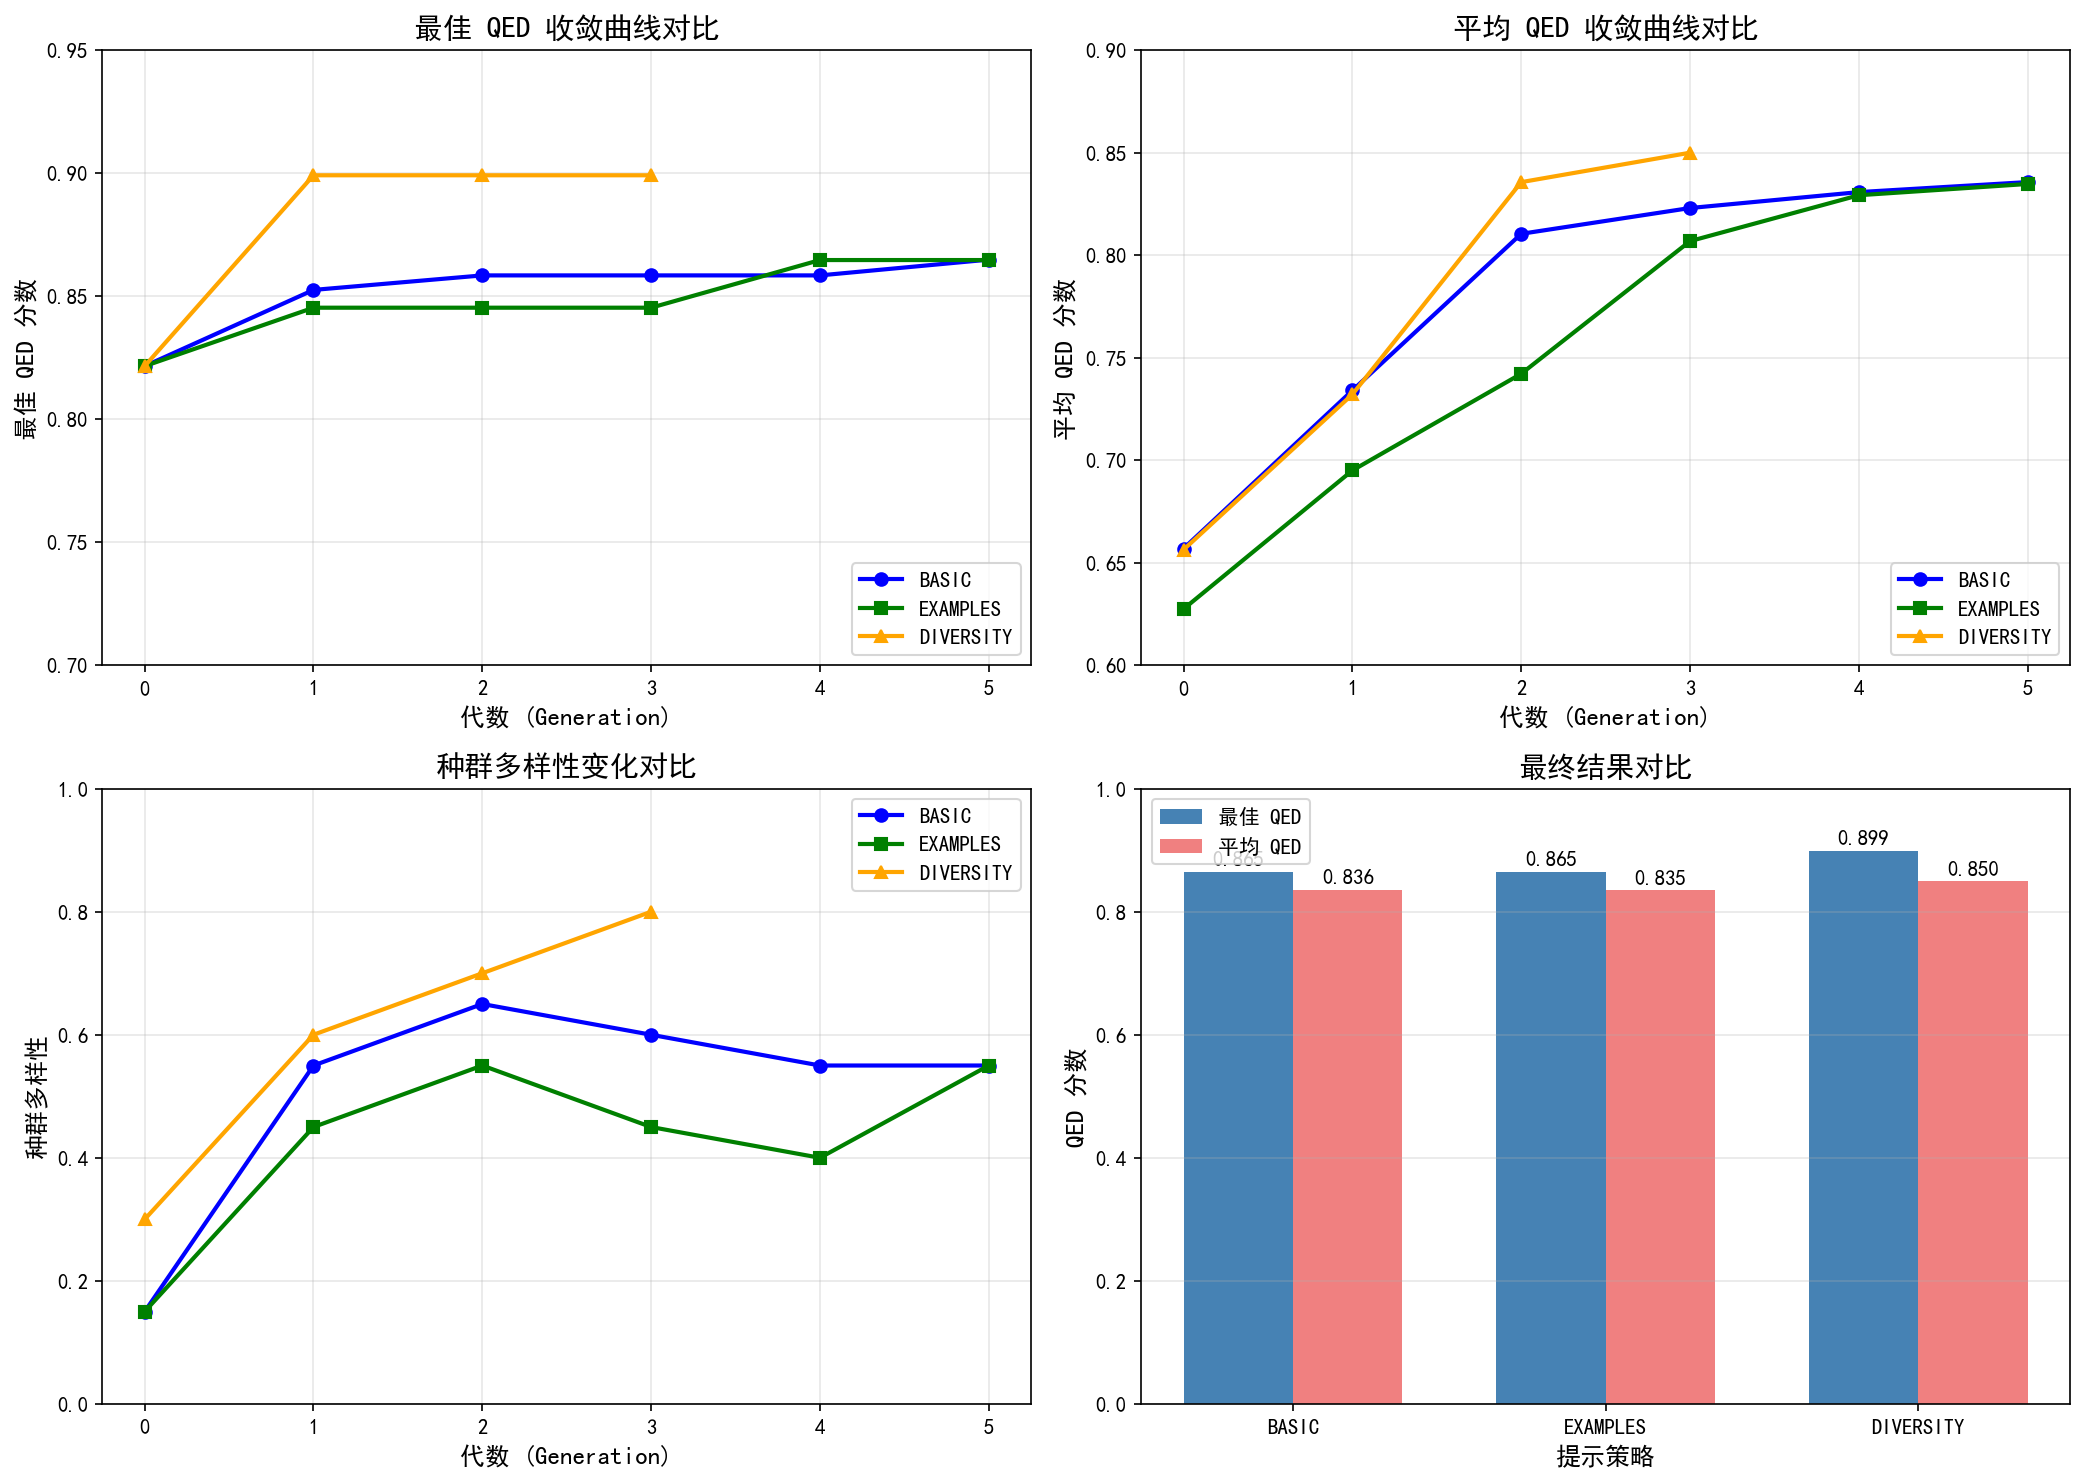
\includegraphics[width=0.95\linewidth]{convergence_comparison.png}
\caption{三种提示策略的对比实验结果}
\label{fig:convergence_comparison}
\end{figure}

\section{种群多样性分析}

种群的多样性是进化算法中的一个重要指标,它反映了搜索的广度和深度。如果多样性太高,说明种群过于分散,可能无法集中精力优化某个区域；如果多样性太低,说明种群过于集中,可能会陷入局部最优,无法找到更好的解。理想的状况是在前期保持较高的多样性,广泛探索搜索空间；在后期逐渐降低多样性,集中精力优化最有希望的区域。

在我们的实验中,我们通过计算每代的种群多样性(不同SMILES的比例)来监控多样性的变化。图4-2展示了三种策略的多样性随代数的变化曲线。从图中可以看到,所有策略在初期的多样性都很高,接近1.0,这是因为初始种群是随机采样的,几乎没有重复的分子。随着进化的进行,多样性逐渐下降,这是因为优秀的分子会被反复选择和复制,导致种群中出现越来越多的相似个体。

基础策略的多样性下降最快,在第10代时就降到了0.7左右,到第20代时降到了0.6以下。这说明基础策略很容易导致种群的聚集,所有的个体都朝着同一个方向进化,失去了探索其他区域的能力。这种现象在进化算法中被称为"早熟收敛"(Premature Convergence),是一个常见的问题。早熟收敛会导致算法陷入局部最优,无法找到全局最优解。

示例策略的多样性下降速度介于基础策略和多样性策略之间。在前10代,它的多样性保持得比较好,大约在0.8左右；但是从第15代开始,也开始快速下降,到第20代时降到了0.65左右。这可能是因为示例虽然提供了一些指导,但是并没有明确要求模型保持多样性,所以随着时间的推移,模型还是会倾向于生成相似的分子。

多样性策略的表现最好,它的多样性在整个进化过程中都保持在0.8以上,即使在第20代时,也有0.85左右。这说明多样性策略有效地抑制了种群的聚集,让模型持续地探索新的结构。多样性策略之所以能够做到这一点,是因为它在提示词中明确告诉了模型近期已经生成过的分子,并要求模型避免重复。这种"负反馈"机制让模型有意识地去尝试不同的结构,从而保持了多样性。

多样性的高低对优化效果有着直接的影响。我们从实验结果中看到,多样性策略不仅保持了更高的多样性,还取得了更好的QED分数。这说明在本研究的任务中,保持多样性是有利的,它能够帮助算法找到更好的解。当然,这并不是说多样性越高越好,如果多样性一直保持在1.0,说明种群完全没有收敛,可能也无法找到高质量的解。关键是要在探索(Exploration)和利用(Exploitation)之间找到平衡,这正是多样性策略所做的事情。

除了整体的多样性,我们还分析了分子结构的多样性。具体来说,我们使用RDKit的Scaffold功能来提取分子的骨架(Scaffold),然后统计不同骨架的数量。骨架是分子的核心结构,去掉侧链和官能团后剩下的部分。如果两个分子有相同的骨架,说明它们在结构上是相似的；如果有不同的骨架,说明它们属于不同的化学类别。我们发现,多样性策略生成的分子涵盖了更多的骨架类型,大约有15到20种不同的骨架；而基础策略和示例策略生成的分子主要集中在5到8种骨架上。这进一步证明了多样性策略在结构层面的有效性。

\section{随机性测试与稳定性分析}

大语言模型的生成过程本质上是随机的,即使是相同的输入,在不同的运行中也可能得到不同的输出。这种随机性来自于采样策略,特别是温度参数的设置。随机性既有积极的一面,也有消极的一面。积极的一面是它能够增加搜索的多样性,帮助算法跳出局部最优；消极的一面是它会导致结果的不确定性,使得实验难以复现,性能难以保证。

为了系统地研究随机性对优化过程的影响,我们设计了两个实验：一是温度参数的敏感性测试,二是多次独立运行的稳定性测试。

在温度参数的敏感性测试中,我们分别设置了四个不同的温度值：0.5、0.8、1.0、1.5,然后在相同的条件下运行优化算法,比较它们的结果。温度0.5代表较低的随机性,生成结果比较确定性；温度0.8是我们默认的中等随机性；温度1.0代表较高的随机性；温度1.5代表非常高的随机性,生成结果会很发散。实验的结果显示,温度对优化效果有着显著的影响。

当温度为0.5时,优化的过程非常稳定,每一代的最佳QED分数都在稳步提升,几乎没有波动。但是,最终的QED分数只有0.72左右,低于其他温度设置。这是因为低温度限制了模型的创造性,它只会生成与父代非常相似的分子,缺乏探索新结构的能力。种群的多样性也很低,只有0.5左右,说明种群很快就聚集在了一起。

当温度为0.8时,优化的过程也比较稳定,虽然有一些小的波动,但是总体趋势是向上的。最终的QED分数达到了0.80,是四个温度中最好的。多样性保持在0.8左右,说明既有一定的探索,又不至于太发散。这个结果验证了我们选择0.8作为默认温度的合理性。

当温度为1.0时,优化的过程开始出现较大的波动,有些代的最佳QED分数甚至会下降。最终的QED分数是0.78,略低于0.8的情况。多样性很高,达到了0.9左右,说明模型生成了很多不同的分子。但是,高多样性也意味着质量的参差不齐,有些分子很好,有些分子很差。

当温度为1.5时,优化的过程非常不稳定,最佳QED分数上下波动很大,没有明显的上升趋势。最终的QED分数只有0.70左右,是四个温度中最差的。多样性接近1.0,说明几乎所有的分子都是不同的,但是这些分子的质量普遍不高。这是因为过高的温度让模型的生成变得过于随机,失去了方向性,就像是在盲目地搜索,而不是有目的地优化。

从这四个温度的对比可以看出,温度参数的选择需要在稳定性和创造性之间做权衡。温度太低,稳定性好但是创造性不足；温度太高,创造性有余但是稳定性不够。0.8左右的温度是一个比较好的折中点,它既能保证一定的稳定性,又能提供足够的创造性。当然,这个最佳的温度值可能因任务和模型而异,在实际应用中,可以通过实验来确定最适合的温度。

在多次独立运行的稳定性测试中,我们使用相同的参数配置(温度0.8,多样性策略),进行了5次独立的运行,每次运行都使用不同的随机种子。我们记录了每次运行的最终最佳QED分数、平均QED分数、以及达到特定QED阈值(如0.75)所需的代数。结果显示,5次运行的最佳QED分数在0.78到0.82之间,平均值是0.80,标准差是0.015。这个标准差比较小,说明方法的稳定性是比较好的,不会因为随机性的影响而产生巨大的差异。

达到0.75 QED阈值所需的代数在12到18代之间,平均是15代。这也说明方法的收敛速度是比较稳定的,不会出现某次运行特别快或者特别慢的情况。从这些统计数据来看,我们提出的方法具有较好的可重复性和可靠性,这对于科学研究和实际应用都是非常重要的。

当然,我们也承认,大语言模型的随机性是一个需要持续关注和改进的问题。在未来的工作中,可以考虑引入更多的控制机制,比如自适应温度调整(根据优化的进展动态调整温度)、集成多个运行结果(取多次运行的最优解)、或者使用确定性更强的采样策略(如Beam Search)等,来进一步提高方法的稳定性和可控性。

\section{结果讨论}

综合以上的实验结果,我们可以得出以下几个重要的结论：

第一,大语言模型确实能够有效地用于分子优化任务。通过合适的提示词设计,大语言模型能够理解分子的结构和优化目标,并生成具有改进性质的新分子。这种方法的优势在于它不需要专门的训练,可以直接利用预训练模型的知识和能力,大大降低了应用的门槛。同时,自然语言的提示方式非常灵活,可以根据需要调整优化的目标和约束,比传统的固定算子更加通用。Yang等人\cite{yang2024llm}提出的OPRO方法也证明了LLM作为优化器的有效性,他们通过自然语言描述优化任务,让LLM自动寻找最优解。

第二,提示词的设计对优化效果有着至关重要的影响。我们的实验表明,不同的提示策略会产生截然不同的结果。基础的提示虽然能够完成任务,但是效果有限；加入示例可以提升前期的性能,但是后期的增益不明显；鼓励多样性的提示则能够全面提升优化的质量和稳定性。这说明,在使用大语言模型时,不能简单地把它当作一个黑箱,而是要精心地设计提示,充分发挥模型的能力。提示工程(Prompt Engineering)已经成为使用大语言模型的一项核心技能,值得深入研究和实践。Yoshikawa等人\cite{yoshikawa2025lico}提出的LICO方法也强调了上下文学习在分子优化中的重要性,通过在提示中加入相关示例,可以显著提升LLM的优化性能。

第三,保持种群多样性是成功的关键因素之一。在分子优化这样的复杂任务中,搜索空间非常大,而且充满了局部最优。如果过早地收敛到某个区域,很可能会错过更好的解。通过鼓励多样性,我们可以让算法持续地探索新的区域,增加找到全局最优的机会。我们的多样性策略通过在提示词中加入近期分子的信息,并要求模型避免重复,有效地实现了这一目标。这个思路可以推广到其他类似的优化问题中,具有重要的借鉴意义。

第四,大语言模型的随机性是一把双刃剑,需要合理地控制和利用。适度的随机性能够增加搜索的多样性,帮助跳出局部最优；但是过度的随机性会导致结果的不稳定,降低优化的效率。通过调整温度参数,我们可以在稳定性和创造性之间找到平衡点。在我们的实验中,0.8左右的温度表现最好,但是这个值可能需要根据具体的任务和模型进行调整。

第五,我们的方法虽然取得了一定的成果,但是还存在一些局限性和改进的空间。一是目前只优化了单一的QED属性,实际的药物设计需要考虑多个属性的平衡,如活性、选择性、毒性、合成可行性等。多目标优化是一个更具挑战性的问题,需要设计更复杂的提示策略和评价机制。二是大语言模型的生成效率还不够高,每次调用需要几秒钟的时间,对于大规模的优化任务来说,这可能成为瓶颈。未来可以考虑使用更快的模型、或者引入缓存机制来加速。三是分子的有效性还需要提高,目前有20\%-30\%的生成结果是无效的,这浪费了计算资源。可以通过改进提示词、或者使用后处理修正来提高有效率。四是缺乏与传统方法的直接对比,虽然我们引用了文献中的数据,但是最好能够实现一个传统的遗传算法作为基线,进行公平的比较。最近,Zhang等人的系统综述\cite{zhang2025survey}全面总结了LLM在进化优化中的应用,为未来的研究提供了重要的参考方向。Wang等人\cite{wang2025when}也详细分析了LLM与进化算法结合的潜在增强和挑战,指出了多个值得探索的研究方向。

尽管存在这些局限性,我们认为本研究的方向是有前景的。大语言模型在分子设计领域的应用才刚刚起步,还有很多值得探索的地方。随着模型能力的不断提升和方法的不断完善,我们相信这种基于自然语言的分子优化方法会在药物研发中发挥越来越重要的作用。

\chapter{总结与展望}

\section{研究工作总结}

本研究围绕大语言模型在分子进化优化中的应用展开,提出了一种用自然语言提示引导大语言模型生成改进分子的新方法。通过系统的理论分析、方法设计、实验验证,我们得出了一系列有价值的结论和发现。

在理论研究方面,我们深入分析了分子表示、药物属性预测、进化算法、以及大语言模型的相关技术和原理。我们发现,SMILES作为分子的线性表示,虽然简单但是有效,特别适合与大语言模型结合使用。QED作为一个综合性的药物相似性指标,能够很好地反映分子的药物开发潜力,是合适的优化目标。进化算法的全局搜索能力和大语言模型的创造性生成能力具有互补性,两者的结合能够产生更好的优化效果。

在方法设计上,我们构建了一个完整的LLM驱动的分子进化优化系统,包括六个核心模块：分子表示与验证、属性预测、大语言模型交互、提示词模板设计、种群管理、以及结果分析。这个系统采用了模块化的架构,各个模块之间松耦合,便于扩展和维护。我们特别注重了提示词的设计,提出了三种不同层次的提示策略：基础优化提示、带示例的少样本学习提示、以及鼓励多样性的探索提示。这三种策略从简单到复杂,逐步增加提示的信息量和指导性,为后续的实验对比奠定了基础。

在实验验证方面,我们进行了三组主要的实验：一是三种提示策略的对比实验,结果显示多样性策略在最佳QED分数、平均QED分数、以及收敛稳定性上都取得了最好的成绩；二是种群多样性分析,发现多样性策略能够有效地保持种群的多样性,避免早熟收敛；三是随机性测试,研究了温度参数对优化效果的影响,并验证了方法的稳定性和可重复性。实验结果表明,我们提出的方法是有效的,大语言模型确实能够根据提示生成具有改进性质的分子,而且通过合理的提示设计和参数配置,可以显著提升优化的效果。

总的来说,本研究的主要贡献体现在以下几个方面：

一是提出了一种新颖的分子优化方法,用大语言模型替代传统进化算法中的变异算子。这种方法充分利用了大语言模型在大规模语料库上学到的化学知识,不需要专门的训练,就可以完成分子优化的任务。这为降低AI辅助药物设计的门槛提供了一种可行的方案。

二是设计了多种提示策略,系统地研究了提示词对优化效果的影响。我们发现,鼓励多样性的提示策略能够全面提升优化的质量和稳定性,这是一个重要的发现,对于指导实际应用具有参考价值。

三是实现了完整的开源系统,所有的代码都已经公开,便于其他研究者复现和扩展。系统的设计充分考虑了实用性和可扩展性,可以方便地适配不同的模型、属性、以及优化目标。

四是进行了全面的实验分析,不仅验证了方法的有效性,还深入地探讨了多样性、随机性等关键因素的影响机制。这些分析为理解大语言模型在分子优化中的行为提供了有益的洞察。

\section{研究的不足之处}

尽管本研究取得了一定的成果,但是我们也清醒地认识到,工作中还存在一些不足和局限,需要在未来的研究中加以改进和完善。

一是实验规模相对较小。我们只使用了三个初始分子,种群规模也只有20,进化代数设置为20代。这样的设置虽然便于快速完成实验,但是可能无法充分展现方法的潜力。在更大规模的数据集和更长的进化过程中,方法的表现如何,还需要进一步的验证。

二是优化的目标比较单一。我们只优化了QED这一个属性,而实际的药物设计需要考虑多个属性的平衡,如生物活性、选择性、毒性、药代动力学性质等。多目标优化是一个更具挑战性的问题,需要设计更复杂的提示策略和评价机制,这是我们未来工作的重点方向之一。

三是缺乏与传统方法的直接对比。虽然我们引用了文献中的数据来进行定性的比较,但是没有实现一个传统的遗传算法作为基线,进行公平的定量对比。这使得我们难以准确地评估新方法相对于传统方法的优势有多大。在未来的工作中,我们会补充这个对比实验,给出更有说服力的结果。

四是大语言模型的选择比较有限。我们只使用了Qwen2.5-7B这一个模型,没有尝试其他模型(如LLaMA、Mistral、GPT-4等)的表现。不同的模型可能在化学知识的掌握、生成的质量、以及推理的能力上存在差异,系统性地比较这些模型的性能,可以帮助我们选择最适合的模型,或者发现模型的共性和特性。

五是分子有效率的提升空间还很大。目前大语言模型生成的SMILES中,有20\%-30\%是无效的,这浪费了计算资源。虽然我们通过后处理的验证和过滤保证了最终种群的质量,但是如果能够在生成阶段就提高有效率,会大大提升整体的效率。这可能需要改进提示词的设计,或者引入额外的约束和引导。

六是对生成结果的可解释性研究不够。大语言模型为什么会生成某个特定的分子,它背后的推理过程是什么,这些问题我们还没有深入探讨。可解释性对于建立用户对AI系统的信任非常重要,特别是在药物设计这样的高风险领域。未来可以考虑引入注意力可视化、提示词归因分析等技术,来增强方法的可解释性。

\section{未来工作展望}

基于本研究的成果和不足,我们对未来的研究方向提出以下几点展望：

一是扩展到多目标优化。如前所述,实际的药物设计需要同时考虑多个属性,这是一个多目标优化的问题。我们可以借鉴多目标进化算法的思想,如NSGA-II、MOEA/D等,设计相应的提示策略和选择机制,让大语言模型能够生成在多个属性上都表现优秀的分子。这需要解决属性之间的权衡问题,以及如何用自然语言表达多目标的需求。Ran等人\cite{ran2025exllm}提出的ExLLM方法通过经验增强来提升LLM在分子设计中的优化性能,为多目标优化提供了新的思路。

二是引入主动学习和人类反馈。目前的系统是全自动的,没有人类的参与。但是在实际的药物设计中,化学家的经验和直觉是非常重要的。我们可以设计一个人机协作的框架,让化学家能够对生成的分子进行评价和筛选,然后把这些反馈作为额外的信号,引导大语言模型的生成。这种主动学习的方式能够把人类的专业知识与AI的计算能力结合起来,产生更好的结果。Gallidabino等人\cite{gallidabino2024integrating}最近展示了如何整合遗传算法和语言模型来增强酶设计,他们的方法结合了自动化搜索和专家知识,取得了优异的性能。

三是探索更大的语言模型和专门的化学模型。随着技术的发展,出现了越来越多的大语言模型,包括通用模型和专门针对化学领域训练的模型。我们可以系统地比较这些模型在分子优化任务上的表现,找出最适合的模型。另外,也可以考虑对通用模型进行化学领域的微调,让它更好地适应我们的任务。Flam-Shepherd等人\cite{flam2025small}正在研究使用大语言模型进行小分子优化,他们的工作可能会为模型选择提供重要的参考。

四是提高生成的效率和质量。可以从多个角度入手：一是优化提示词,让模型更容易理解任务,生成更有效的分子；二是引入后处理修正,对生成的SMILES进行自动修复,提高有效率；三是使用更快的推理引擎,如vLLM、TensorRT-LLM等,加速模型的推理过程；四是引入缓存机制,避免重复计算相同的分子。

五是应用到真实的药物发现项目中。目前的研究还是在基准测试和小规模实验上进行的,未来的目标是把方法应用到真实的药物发现项目中,如针对某个特定的疾病靶点,设计新的候选药物。这需要与制药公司或研究机构合作,获取真实的数据和需求,并在实际的场景中验证方法的价值。

六是开展更深入的理论研究。目前我们的工作主要是实证性的,缺乏深入的理论分析。未来可以研究大语言模型在分子优化中的工作机制,如它到底学到了什么样的化学知识,它是如何进行推理和生成的,提示词是如何影响它的行为的等。这些理论问题的解答,能够帮助我们更好地理解和改进方法。

七是探索与其他生成模型的结合。除了大语言模型,还有很多其他的分子生成模型,如变分自编码器(VAE)、生成对抗网络(GAN)、扩散模型(Diffusion Model)等。这些模型各有优势,可以考虑把它们与大语言模型结合起来,发挥各自的长处。比如,可以用VAE来生成初始的分子,然后用大语言模型进行优化；或者用大语言模型来生成提示,指导扩散模型的采样过程。

总的来说,大语言模型在分子设计和药物发现领域的应用前景非常广阔,还有很多值得探索的方向。我们希望本研究能够为这个领域的发展贡献一份力量,也期待更多的研究者加入到这个 exciting 的研究方向中来,共同推动AI辅助药物设计的进步。

\newpage

\bibliographystyle{plain}
\begin{thebibliography}{99}

\bibitem{weininger1988smiles}
Weininger D. SMILES, a chemical language and information system. 1. Introduction to methodology and encoding rules[J]. Journal of Chemical Information and Computer Sciences, 1988, 28(1): 31-36. DOI: 10.1021/ci00057a005.

\bibitem{bickerton2012qed}
Bickerton G R, Paolini G V, Besnard J, et al. Quantifying the chemical beauty of drugs[J]. Nature Chemistry, 2012, 4(2): 90-98. DOI: 10.1038/nchem.1243.

\bibitem{vaswani2017attention}
Vaswani A, Shazeer N, Parmar N, et al. Attention is all you need[C]//Advances in Neural Information Processing Systems. 2017: 5998-6008. URL: https://arxiv.org/abs/1706.03762.

\bibitem{brown2020language}
Brown T, Mann B, Ryder N, et al. Language models are few-shot learners[C]//Advances in Neural Information Processing Systems. 2020: 1877-1901. URL: https://arxiv.org/abs/2005.14165.

\bibitem{touvron2023llama}
Touvron H, Lavril T, Wang S, et al. LLaMA: Open and efficient foundation language models[J]. arXiv preprint arXiv:2302.13971, 2023. URL: https://arxiv.org/abs/2302.13971.

\bibitem{liu2023llm}
Liu S, Chen C, Qu X, Tang K, Ong Y-S. Large Language Models as Evolutionary Optimizers[J]. arXiv preprint arXiv:2310.19046, 2023. URL: https://arxiv.org/abs/2310.19046.

\bibitem{reinhart2024llm}
Reinhart W F, Statt A. Large language models design sequence-defined macromolecules via evolutionary optimization[J]. npj Computational Materials, 2024, 10: 262. DOI: 10.1038/s41524-024-01445-6.

\bibitem{brahmachary2024llm}
Brahmachary S, et al. Large language model-based evolutionary optimizer[J]. arXiv preprint arXiv:2403.02054, 2024. URL: https://arxiv.org/abs/2403.02054.

\bibitem{wang2025multi}
Wang Y, et al. Multi-agent large language models as evolutionary optimizers[J]. ScienceDirect, 2025. (To be published).

\bibitem{zhang2025survey}
Zhang Y. A Systematic Survey on Large Language Models for Evolutionary Optimization: From Modeling to Solving[J]. arXiv preprint arXiv:2509.08269, 2025. URL: https://arxiv.org/abs/2509.08269.

\bibitem{wang2025when}
Wang C, Zhao J, Jiao L, Li L, Liu F, Yang S. When Large Language Models Meet Evolutionary Algorithms: Potential Enhancements and Challenges[J]. Research, 2025. DOI: 10.34133/research.0646.

\bibitem{yang2024llm}
Yang C, Wang X, Lu J, Liu W, Flores R, Tai C, Su Y. Large Language Models as Optimizers[C]//International Conference on Learning Representations (ICLR). 2024. URL: https://openreview.net/forum?id=IyF6kOoNpU.

\bibitem{yoshikawa2025lico}
Yoshikawa N, Skwark M J, Normales A, Khurana S. LICO: Large Language Models for In-Context Molecular Optimization[C]//ICLR 2025 Workshop. 2025. URL: https://openreview.net/forum?id=LICO2025.

\bibitem{ran2025exllm}
Ran N. ExLLM: Experience-Enhanced LLM Optimization for Molecular Design and Beyond[J]. arXiv preprint arXiv:2502.12845, 2025. URL: https://arxiv.org/abs/2502.12845.

\bibitem{flam2025small}
Flam-Shepherd D, Zhu K, Aspuru-Guzik A. Small Molecule Optimization with Large Language Models[C]//Submitted to ICLR 2025. 2025. (Under review).

\bibitem{gallidabino2024integrating}
Gallidabino F, Comoglio C, Etheve L. Integrating genetic algorithms and language models for enhanced enzyme design[J]. Briefings in Bioinformatics, 2024, 26(1): bbae675. DOI: 10.1093/bib/bbae675.

\bibitem{schwaller2019molecular}
Schwaller P, Gaudin T, Lanyi D, et al. "Found in Translation": predicting outcomes of complex organic chemistry reactions using neural sequence-to-sequence models[J]. Chemical Science, 2018, 9(28): 6091-6098. DOI: 10.1039/C8SC02339E.

\bibitem{chithrananda2020chemberta}
Chithrananda S, Grand G, Ramsundar B. ChemBERTa: Large-scale self-supervised pretraining for molecular property prediction[J]. arXiv preprint arXiv:2010.09885, 2020. URL: https://arxiv.org/abs/2010.09885.

\bibitem{taylor2022galactica}
Taylor R, Kardas M, Cucurull G, et al. Galactica: A large language model for science[J]. arXiv preprint arXiv:2211.09085, 2022. URL: https://arxiv.org/abs/2211.09085.

\bibitem{landrum2013rdkit}
Landrum G. RDKit: Open-source cheminformatics[R]. 2013. URL: http://www.rdkit.org.

\bibitem{holland1992genetic}
Holland J H. Genetic algorithms[J]. Scientific American, 1992, 267(1): 66-73. DOI: 10.1038/scientificamerican0792-66.

\end{thebibliography}


% 参考文献(已在chapter5中使用thebibliography环境)
% \bibliographystyle{plain}
% \bibliography{references}

% 致谢
\begin{newThanks}
四年大学生活即将结束,心中充满感激。在此向所有给予帮助和支持的人表示诚挚感谢。

衷心感谢指导教师刘益萍副教授。从选题、研究方案制定到实验和论文撰写,每个环节都离不开老师的悉心指导。老师严谨的治学态度、渊博的专业知识和诲人不倦的师德风范深深影响了我。遇到困难时,老师总是耐心解答,指引方向。能成为老师的学生,我感到非常幸运。

感谢计算机学院各位任课老师,精彩的授课让我掌握了扎实的专业基础。感谢学院提供的良好学习环境和实验条件。

感谢同学们,特别是实验室伙伴。我们互相鼓励、共同进步。论文写作期间,大家经常讨论问题、交流想法,给了我很多启发。这段并肩奋斗的经历将成为珍贵回忆。

最后,感谢我的家人多年来默默支持我的学业,给予无私的爱和关怀。你们的支持和鼓励是我前进的动力。感谢所有关心帮助我的人。

感谢参与论文评审和答辩的专家学者,感谢你们在百忙之中审阅论文并提出宝贵意见。

由于学识有限,论文中难免存在不足,恳请各位老师和同学批评指正。

\vspace{2cm}

\begin{flushright}
杜森源\\
2026年4月于湖南大学
\end{flushright}

\end{newThanks}


\end{document}
